%%%%%%%%%%%%%%%%%%%%
\chapter{Equilibrium Interface models and their finite size effects}
%%%%%%%%%%%%%%%%%%%%

Models for interfaces arise naturally in phase separated systems, as explained in \ref{chap-int-dyn}. Finite size corrections are manifested when the correlation length becomes of the order of magnitude of the system's size. When undergoing a continuous phase separation, the system exhibits finite size corrections which are manifested by a long range critical Casimir interaction, which we describe in the first section. In the second section we examine finite size effects in continuous interface models in one dimension, and show that while they have similar long-range interactions, the forces induced by interface confinement are quite different, and will be compared to the GSOS model. In the last section, we compute the size-dependent eigenvalues of the transfer matrix for the free SOS model, and compare the results with previous works.

%%%%%%%%%%%%%%%%%%%%
\section{The Casimir effect}
\label{sec-casimir}
%%%%%%%%%%%%%%%%%%%%

Here we explain the critical Casimir effect. For completeness we start by explaining the quantum Casimir effect as it was in the quantum context that the effect was first observed \cite{h_b_g_casimir_attraction_1948}.
We also describe the basis of the Lifshitz theory that generalises Casimir's contribution to 
general dielectric materials beyond the perfectly conducting plate paradigm.

%%%%%%%%%%%%%%%%%%%% 
\subsection{Quantum Casimir effect}
%%%%%%%%%%%%%%%%%%%%
In an ideal conductor, the free charges can move arbitrarily quickly to cancel out any electric in the plane \cite{richard_feynman_feynman_1963}. Thus, a perfectly conducting plate in the $(x,y)$ plane imposes boundary conditions on the electromagnetic field
\begin{equation}
{\bf E}\times {\bf n} = {\bf 0};\ {\bf B}\cdot {\bf n} = 0
\end{equation}
The quantum Hamiltonian for the electromagnetic field is given by 
\begin{equation}
H = \sum_{\bk,\lambda}\hbar \omega(\bk,\lambda)\left[a^\dagger(\bk,\lambda)a(\bk,\lambda) + {1\over 2}\right]
\end{equation}
Here $\lambda$ denotes the polarisation (there are two polarisation states) and $\bk$ the wave vector. The dispersion 
relation for photons is
\begin{equation}
\omega(\bk,\lambda) = |\bk|c.
\end{equation}
The ground state energy of the electromagnetic field \cite{h_b_g_casimir_attraction_1948} is given by
\begin{equation}
E_0 = < 0|H|0> = H = \sum_{\bk,\lambda}{1\over 2}\hbar \omega(\bk,\lambda)= \sum_\bk\hbar |\bk|c
\end{equation}

The presence of conduction plates at $z=0$ and $z=L$ means that the wave vectors $k_z$
must be quantised according to $k_z= n\pi/L$ where $n \in \{0,\ 1, \ 2, \ \cdots\}$ while
if the $(x,y)$ plane has a large area $A$ we can write
\begin{equation}
\sum_{k_x,k_y}\ \cdot= {A\over (2\pi)^2}\int d^2\bk \ \cdot
\end{equation}
This then gives 
\begin{eqnarray}
E_0(L) &=& {\hbar c A\over (2\pi)^2}\sum_{n=0}^\infty \int d^2\bk \left(\bk^2 + {n^2\pi^2\over L^2}\right)^{1\over 2} \\
&=& {\hbar c A\over (2\pi)}\sum_{n=0}^\infty \int_0^\infty kdk \left(\bk^2 + {n^2\pi^2\over L^2}\right)^{1\over 2}
\end{eqnarray}
The problem with the above expression is that it is clearly divergent. However it can be rendered finite by cutting off the high momentum degrees of freedom by writing
\begin{equation}
E_0(L) = {\hbar c A\over (2\pi)}\sum_{n=0}^\infty \int_0^\infty kdk \left(\bk^2 + {n^2\pi^2\over L^2}\right)^{1\over 2} f\left((\bk^2 + {n^2\pi^2\over L^2})^{1\over 2}\right)
\end{equation}
where $f$ is a smooth function such that $f(p)=1$ for $p\ll\Lambda$ and $f(p)=0$ for $p\gg\Lambda$. Here, $\Lambda$ is an ultraviolet cut-off and $f$ thus only counts the contribution of photons with a momentum less than $\hbar\Lambda$. For this sort of calculation to make physical sense the physical result we get at the end should be independent of both the choice of $f$ and $\Lambda$. 




In the limit $L\to\infty$ we can replace the sum over discrete modes by an integral, as usual in statistical physics, 
\begin{equation}
E_0(L) = {\hbar c A\over (2\pi)}\int_{0}^\infty {L\over \pi}d\nu \int_0^\infty kdk \left(\bk^2 + \nu^2\right)^{1\over 2}f\left((\bk^2 + \nu^2)^{1\over 2}\right)
\end{equation}
where we have used $d\nu = \pi/L$. We thus see that for large $L$ we have
\begin{equation}
E_0(L) = AL \epsilon_{bulk}
\end{equation}
where $\epsilon_{bulk}$ is a bulk energy density per unit of volume, that is to say the total energy is extensive.  The computation above only calculates the energy of the EM field between the plates. If the physical system extends up to $L'\gg L$, then the total energy of both the interior and the exterior of the plates is
given by
\begin{equation}
E_{total}(L) = E_0(L) + A(L'-L)\epsilon_{bulk}
\end{equation}
We see that the part of the energy that depends on $L$ is given by
\begin{equation}
U(L) = E_0(L)- AL\epsilon_{bulk}
\end{equation}
It is the derivative of $U$ which gives the physical interaction between the two plates, the pressure associated with this interaction in the colloid science literature is called the disjoining pressure \cite{stubenrauch_disjoining_2003} where to compute the effective interaction the bulk pressure has to be subtracted.
Now we simply write 
\begin{equation}
AL\epsilon_{bulk} = {\hbar c A\over (2\pi)}\int_{0}^\infty dn \int_0^\infty kdk \left(\bk^2 + {n^2\pi^2\over L^2}\right)^{1\over 2} f\left((\bk^2 + {n^2\pi^2\over L^2})^{1\over 2}\right)
\end{equation}
where we have put the $L$ dependence in the integral. This then gives
\begin{equation}
U(L) = {\hbar c A\over (2\pi)}\left[\sum_{n=0}^\infty g(n) -\int_0^\infty dn \ g(n)\right]
\end{equation}

where
\begin{equation}
g(n) = \int_0^\infty kdk \left(\bk^2 + {n^2\pi^2\over L^2}\right)^{1\over 2} f\left((\bk^2 + {n^2\pi^2\over L^2})^{1\over 2}\right) = {1\over 2}\int_{n^2\pi^2\over L^2}^\infty du u^{1\over 2} f(u^{1\over 2})
\end{equation}
We now use the Euler-Mauclarin formula
\begin{equation}
\sum_{n=0}^\infty g(n) -\int_0^\infty dn \ g(n) = -B_1g(0) -{1\over 2} B_2 g'(0) - {1\over 24} B_4 g'''(0) - \cdots
\end{equation}
where $B_n$ are the Bernoulli numbers\footnote{The first Bernoulli numbers are explicitly given by $B_1 =1\ , B_2 = {1\over 2} ,\ B_4 = -{1\over 30}$}.
We find that
\begin{equation}
g'(n) = -{\pi^3\over L^3} n^2 f({n\pi\over L})
\end{equation}
and noticing than in the region around $n=0$, $f=1$ is a constant, we show that
\begin{eqnarray}
g'(0) &=& 0 \\
g''(0) &=& 0 \\
g'''(0) &=& -{2\pi^3\over L^3}
\end{eqnarray}
Higher order derivatives are zero so the full result is given by the first three terms of the Euler-Maclaurin formula. We thus find
\begin{equation}
U(L) = {\hbar c A\over (2\pi)}\left[ -g(0) -{\pi^3\over 360 L^3}\right]
\end{equation}
The first term independent of $L$ can be interpreted as a surface energy. The effective $L$ dependent interaction is given by
\begin{equation}
U_{int}(L) = -{\hbar \pi^2 c A\over 720 L^3}
\end{equation}
We see that the effective interaction is attractive. Interestingly Casimir thought that his calculation could explain the stability of the electron \cite{h_b_g_casimir_attraction_1948,carazza_casimir_1986} The model of the electron is one of a perfectly conducting shell carrying an electric charge $e$. If the radius of the shell is $a$ then the electrostatic energy of due to the charge is given by
\begin{equation}
E_{Charge} = {e^2\over 8\pi a\epsilon_0}
\end{equation}
There is thus a repulsive force on the shell which should make it expand. Casimir thought that the Casimir force on a spherical geometry, 
if is an attractive force as is the case for the parallel plate geometry, could stabilise the electron. Clearly by dimensional analysis
\begin{equation}
E_{Cas} = -{Z\hbar c\over a}
\end{equation}
The balance of the Casimir and electric forces would then require
\begin{equation}
Z = {e^2\over 8\pi \hbar c}.
\end{equation}
However, in the case of conducting spherical shell, the constant $Z \simeq -0.046175$ is negative \cite{boyer_quantum_1968,milton_casimir_1978,bowers_casimir_1998}, while the same calculation for a cylindrical geometry predicts an attractive force \cite{milton_casimir_1978-1}. 

%%%%%%%%%%%%%%%%%%%%
\subsection{Lifshitz Theory}
%%%%%%%%%%%%%%%%%%%%
The Casimir calculation is based on the boundary conditions imposed on the EM field 
due to a conductor. However, this is an ideal mathematical limit, conductors being conductors because free charges can move to cancel out the electric field in the conducting surface.
The Casimir force can also be seen as due to correlations induced in the charge fluctuations in each plate, which allows for an alternative method based on sources which recovers the Casimir force \cite{julian_schwinger_casimir_1978,schwinger_casimir_1992}. In a sense therefore the effect can be interpreted without reference to the zero point energy of the vacuum and the Casimir calculation works due to the fact that the mathematical limit in going to a perfect conductor works. 
Using a stochastic formulation of electrodynamics by Rytov \cite{sm_rytov_principles_1989}, the Casimir calculation was generalized by Lifshitz for interactions between arbitrary electrical bodies, characterized by their local electric and magnetic response\cite{lifshits_theory_1955}. 
Even though this theory is very general, the microscopic justification is not completely rigorous, source terms (random currents and dipole fluctuations) are introduced to Maxwell's equations to give a Langevin formulation of Maxwell's equations in the presence of dielectric bodies. The correlation functions of the white noise terms depend on the temperature of the system and are determined via the quantum fluctuation dissipation theorem. The Lifshitz theory is computationally difficult to work with and it was reformulated in a way more useful for practical calculations and that can be applied to experimental setups \cite{van_kampen_macroscopic_1968,ninham_van_1970}.
Rytov's formulation has the advantage that it can be used to treat out of equilibrium situations where different bodies are held at different temperatures. This allows both the computation of out of equilibrium forces and radiative heat transfer. 

The theory in the presence of electromagnetic media is written in terms of the electric and magnetic fields ${\bf E}$ and ${\bf B}$ and the displacement and magnetizing fields ${\bf D}$ and ${\bf H}$ which are assumed to obey local relations in real space and Fourier space
\begin{equation}
\tilde {\bf D}(\omega)=\epsilon(\omega)\tilde{\bf E}(\omega); \ \tilde {\bf B}(\omega)= \mu(\omega) \tilde{\bf H}(\omega)
\end{equation}
where $\tilde\epsilon( \omega)$ and $\tilde\mu( \omega)$ are the frequency dependent
permittivity and permeability. The boundary conditions at the interface between two materials $1$ and $2$ are given by
\begin{eqnarray}
B_{1n}= B_{2n} && \ D_{1n}=D_{2n} \\
E_{1t} = E_{2t} && \ H_{1t}=H_{2t}
\end{eqnarray}
where $n$ denotes the normal component and $t$ the tangential component to the interface.

Forces can be computed using the vacuum (assuming that the surface where the force is computed is next to the vacuum) Maxwell stress tensor.
\begin{equation}
T_{ij}= \epsilon\left(E_iE_j -{1\over 2}\delta_{ij}E^2\right) + {1\over \mu}\left( B_i B_j -{1\over 2}\delta_{ij}B^2\right)
\end{equation}
Notice that the stress tensor is quadratic in the fields ${\bf E}$ and ${\bf B}$, this means that even if the fields are on average zero, both thermal and quantum fluctuations give rise to forces.

In media Maxwells equations are
\begin{eqnarray}
\nabla \times{\bf E} &=& -{\partial {\bf B}\over \partial t} \\
\nabla \times{\bf H} &=& {\bf J}-{\partial {\bf D}\over \partial t} \\
\nabla \cdot {\bf D} &=& \rho\\
\nabla \cdot {\bf B} &=& 0 
\end{eqnarray}

In a dielectric medium or conductor where there are no applied external fields there is no free charge or current . As such, the average values of ${\bf E}$ and ${\bf B}$ are zero. Rytov's idea was to add a random current to induce both thermal and quantum fluctuations
into the problem. If we assume that the only contribution to the current comes from a fluctuating polarization density ${\bf P}$ we can write
\begin{equation}
{\partial \rho\over \partial t} +\nabla \cdot {\bf J}= 0\implies\nabla\cdot \left[-{\partial {\bf P}\over \partial t} +{\bf J}\right] = 0
\end{equation}
where we have used
\begin{equation}
\rho = -\nabla \cdot {\bf P}
\end{equation}
This means that the current is given by
\begin{equation}
{\bf J}={\partial {\bf P}\over \partial t} 
\end{equation}
or in Fourier space
\begin{equation}
\tilde {\bf J}(\omega)= i\omega \tilde P(\omega)
\end{equation}
Now if we assume that the fluctuations in the polarization density are uncorrelated in space, the fluctuation dissipation theorem tells us that the correlation function of the polarization density in Fourier space is given by
\begin{equation}
< P_\alpha(\omega; \bx)P^{\dagger}_\beta(\omega; \bx')>_{sym}=
{\hbar \epsilon''(\omega)\over 2}\coth\left({\hbar\omega\over 2k_B T}\right)\delta(\omega-\omega')\delta(\bx-\bx')\delta_{\alpha\beta}
\end{equation}

\begin{equation}
\epsilon(\omega) = \epsilon'(\omega)+i\epsilon''(\omega)
\end{equation}
The Lifshitz calculation for slab geometries gives a force per unit area between two slabs of media separated by a distance $L$
\begin{eqnarray}
{F\over A} &=& -{k_BT \over \pi c^3}\sum_{n=0}^\infty \omega_n^3 \int_1^\infty dp p^2 \ 
\left[ 1-{(s_1+p)(s_2+p)\over (s_1-p)(s_2-p)}\exp(-{2p\omega_n L\over c})\right]\nonumber \\
&+&\left[ 1-{(s_1+p\varepsilon_1)(s_2+p\varepsilon_2)\over (s_1-p\varepsilon_1)(s_2-p\varepsilon_2)}\exp(-{2p\omega_n L\over c})\right]
\end{eqnarray}
where $\epsilon = \epsilon_0\varepsilon$, $s_i = \sqrt{\epsilon_i -1 +p^2}$,
$\omega = {2\pi nk_BT \over \hbar}$ are the Mastubara frequencies \cite{matsubara_new_1955} and ${\varepsilon_i
=\varepsilon_i(i\omega_n)}$. Note that the integral over real frequencies has become a sum over discrete Matsubara frequencies, they come from the poles in the hyperbolic cotangent.

One needs to know the dielectric response at imaginary frequency, this is done using the Kramers-Kronig relation
\begin{equation}
\varepsilon(i\omega)= 1 +{2\over \pi}\int_0^\infty d\zeta {\zeta \varepsilon''(\zeta)\over \omega^2 + \zeta^2}
\end{equation}


%%%%%%%%%%%%%%%%%%%%
\subsection{Critical Casimir effect}
%%%%%%%%%%%%%%%%%%%%

{\color{red}
In systems having a continuous phase transition the correlation length diverges as the critical point is approached. This means that the correlation length has a size comparable to that of the system size, this  leads to strong finite-size effects in the free energy. Following the arguments of Fisher and de Gennes \cite{gambassi_casimir_2009}, we describe how a version of  the Casimir effect is manifested in  critical systems. 
}
%%%%%%%%%%%%%%%%%%%%
\subsubsection{Bulk scaling for near critical systems}
%%%%%%%%%%%%%%%%%%%%
The free energy for a system consisting of $N$ spins has a singular part at a critical temperature $T_c$ which can be written as
\begin{equation}
F(t,h) = N f(t,h)
\end{equation}
where $t = (T-T_c)/ T_c$ measures the distance from the critical point and $h$ is the external applied magnetic field. We assume that we are in a system where the only relevant parameters are $T$ and $h$ (equivalently the concentration or chemical potential of a binary mixture), which is true for $d\less 4$ \cite{amit_field_2005}.
Now if we carry out a renormalisation group transformation
blocking spins in blocks of linear size $b$ into new effective spins, the RG transformation
gives
\begin{equation}
N f(t,h) = N'f(t',h')
\end{equation}
Clearly the number of spins in the blocked system is given by $b^d N'=N$ and the RG transformation for $t$ and $h$ are given by $t' = b^{y_1} t$ and $h' = b^{y_2}h$, where $y_1$ and $y_2$ are positive and are the RG exponents for the fields $t$ and $h$ (from which all critical exponents can be deduced). This then means that
\begin{equation}
f(t,h) = {1\over b^d}f(b^{y_1} t, b^{y_2} h) 
\label{rg}
\end{equation}
We begin by working with $t\greater 0$ but the arguments here are trivially generalisable to the case $t\less 0$. In Eq. (\ref{rg}) is we choose $b$ such that $b^{y_1}t=1$, then, at the critical field $h=0$, we find
\begin{equation}
f(t,0) = t^{d\over y_1} f(1,0)
\end{equation}
The singularity in the specific heat is defined via
\begin{equation}
c\sim {\partial^2 \over \partial t^2}f(t,0)
\end{equation}
and so we find
\begin{equation}
c\sim t^{{d\over y_1}-2} \sim t^{-\alpha}
\end{equation}
where $\alpha$ is the exponent associated with the divergence of the specific heat. This means that
\begin{equation}
\alpha = 2 -{d\over y_1}
\end{equation}
The RG transformation for the correlation function has the form
\begin{equation}
C(r,t,h) = \lambda^2(b) C(r/b, b^{y_1}t, b^{y_2} h)
\end{equation}
Clearly length scales transform as $r' = r/b$. Again setting $h=0$ and choosing $b^{y_1}t=1$ gives
\begin{equation}
C(r,t,h) = \lambda^2(t^{-{1\over y_1}}) C(r/t^{-{1\over y_1}}, 1, 0).
\end{equation}
The correlation function, by definition is given by
\begin{equation}
C(r,t) \sim f(r/\xi),
\end{equation}
where $\xi$ is the correlation length. This immediately tells us that $\xi = t^{-{1\over y_1}}$ and from the usual definition 
\begin{equation}
\xi \sim t^{-\nu}
\end{equation}
we have $\nu = 1/y_1$. These two formula for $y_1$ then give the hyper scaling relation
\begin{equation}
\alpha = 2-d\nu.
\end{equation}
The exponents $\alpha$ and $\nu$ are the ones that are important in the critical Casimir effect.

%%%%%%%%%%%%%%%%%%%%
\subsubsection{Finite size scaling}
%%%%%%%%%%%%%%%%%%%%
Consider a system which is finite in one direction with either periodic boundaries or 
two surfaces. While the critical system has $h=0$ there can be local surface fields at each surface $a$ and $b$. This represents a preference of the surfaces for one phase or the other. 
The finite scaling hypothesis for a slab system of large area $A$ but with finite width $L$ can be stated as
\begin{equation}
f(t,h_a,h_b,L^{-1}) = {1\over b^{d}}f(b^{y_1}t, b^{y_a} h_a, b^{y_b} h_b, bL^{-1}) \label{ffs}
\end{equation}
We thus see that the field $L^{-1}$ is a relevant field with RG exponent $y_L=1$. 
The surface fields are not necessarily relevant so we can have $y_a$ and $y_b$ positive or negative. The important point about finite size scaling is that when $L$ is finite the singularity due to the thermodynamic phase transition is smoothed out by the system's finite size (note that we assume that the system has no two-dimensional phase transition in the region we are looking at). First we see that when $L$ is large there should be a bulk contribution to the free energy plus a surface term (so we are considering the limit $L\to\infty$ before $\xi\to\infty$)
\begin{align}
f(t,h_a,h_b,L^{-1}) =& f(t,h_a,h_b,0) + L^{-1}{\partial f(t,h_a,h_b,0)\over \partial x_4} \nn
=& {1\over b^d} f(b^{y_1}t, b^{y_a} h_a, b^{y_b} h_b,0)+{1\over b^{d-1}}L^{-1}{\partial f(b^{y_1}t, b^{y_a} h_a, b^{y_b} h_b, 0)\over \partial x_4}
\end{align}
where we have carried out the Taylor expansion for $L^{-1}$ small using both versions of Eq. (\ref{ffs}) and ${\partial \over \partial x_n}$ indicates the partial derivative with respect to the $n^{th}$ argument. 
The second term gives a total contribution to the singular part of the free energy of the order $AL \times L^{-1}$ and is thus a surface tension $\gamma$ and so we have
\begin{equation}
\gamma= {1\over b^{d-1}}{\partial f(b^{y_1}t, b^{y_a} h_a, b^{y_b} h_b, 0)\over \partial x_4}
\end{equation}


Setting $bt^{y_1}=1$ then gives close to the critical point
\begin{equation}
\gamma \sim t^{d-1\over y_1}{\partial f(1,\lim_{t\to 0} t^{-\frac{y_a}{y_1}}h_a, \lim_{t\to 0} t^{-\frac{y_a}{y_1}}h_b,0)\over \partial x_4} = t^{(d-1)\nu}C' = \xi^{-(d-1)}C'
\end{equation}
The formula relating the surface tension and the correlation length, in the above $C'$ is a constant depending on the universality class. 

Now if we keep $L$ finite and set $b^{y_1}t=1$ in Eq. (\ref{ffs}) we find
\begin{equation}
f(t,h_a,h_b,L^{-1}) = t^{d\over y_1}f(1, t^{-{y_a\over y_1}} h_a, t^{-{y_b\over y_1}} h_b, t^{-{1\over y_1}}L^{-1})
\label{ffs}
\end{equation}
which can be written as
\begin{equation}
f(t,h_a,h_b,L^{-1}) = {1\over \xi^d}f(1,\xi^{y_a} h_a, \xi^{y_b} h_b, \xi/L)
\end{equation}
This can then be written as
\begin{equation}
f(t,h_a,h_b,L^{-1}) = {1\over L^d}\theta({L\over \xi}, \xi^{y_a} h_a, \xi^{y_b} h_b)
\end{equation}
Now crucially as $\xi \to \infty$ the function $\theta$ is analytic so we can take the limit $\xi\to\infty$ without any problems to find
\begin{equation}
f(0,h_a,h_b,L^{-1}) = {1\over L^d}\theta(0, \lim_{\xi\to \infty} \xi^{y_a} h_a,\lim_{\xi\to \infty} \xi^{y_b} h_b)
\end{equation}
Clearly for each surface we have 3 possibilities: $\lim_{\xi\to \infty} \xi^{y_a} h_a = \pm \infty$, if the surface fields are relevant, as well as $\lim_{\xi\to \infty} \xi^{y_a} h_a = 0$ if the surface fields are irrelevant. There is clearly also a similar argument when the system has periodic boundary conditions and there are no surface fields. Near the critical point depending on the boundary conditions there should be scaling functions when the surface fields attract the same phase $\theta_{++}(x)$, where they attract different phases and
$\theta_{+-}(x)$, and $\theta_{pbc}(x)$ when the boundary conditions are periodic. There should also be a zero surface field case $\theta_{00}$ when the surfaces fields are irrelevant or zero (this is however unlikely). Fisher and de Gennes argued, without proof, that the force for $(++)$ boundary conditions should be attractive where as the $(+-$) case should produce repulsive forces \cite{gambassi_casimir_2009,gambassi_critical_2009} . 

The total singular part of the free energy is thus given by
\begin{equation}
F = ALf(t,h_a,h_b,L^{-1}) = {A\over L^{d-1}}\theta({L\over \xi}, \xi^{y_a} h_a, \xi^{y_b} h_b).
\end{equation}

The scale of the energy is set by the energy of thermal fluctuations $k_BT$ we thus find
that 
\begin{equation}
F(t=0) = {k_BT A C\over L^{d-1}}
\label{casfreeenergy}
\end{equation}
where $C$ is a constant depending on the surface universality class.


%%%%%%%%%%%%%%%%%%%%
\section{Finite size scaling in one dimensional interface models}
%%%%%%%%%%%%%%%%%%%%

We have seen that confinement generated Casimir forces appear when the correlation length of the fluctuations in a system becomes of the order of the minimum size of the system,  be it for perfect conductor plates in vacuum or in confined critical systems. We have also seen that interfaces between two phases can described by surface models. If we consider just a surface model, it is physically obvious that finite size effects will also arise in these systems. In what follows we will study the size dependence of a number of continuous and discrete interface models (corresponding to the interfaces of two dimensional systems). While long range forces are generated by confinement we find that these models have quantitatively different behaviours to the critical Casimir effect. However if one assumes a phenomenological proposal by Privman \cite{privman_finite-size_1988-1} to introduce a finite size correction to the surface tension, the critical Casimir effect can be quantitatively recovered.

%%%%%%%%%%%%%%%%%%%%
\subsection{Continuous models in one dimension}
%%%%%%%%%%%%%%%%%%%%

In one dimension the partition function for a surface model of the type discussed in Sec \ref{sec-continuous} can be written as a path integral 
\begin{equation}
Z(t)  = \int d[h]\exp\left(-\frac{\beta\sigma}{2}\int_0^t h'^2(x) dx -\beta\int_0^t  V(h(x)) dx\right)
\end{equation}
where $t$ is the length of the system and the notation is so chosen as the variable $x$ con be thought of as a time in path integral language.
It is convenient to fix both the starting point $h(0)=x$ and the end point $h(t)=x$ and define what is known as the propagator \cite{matsubara_new_1955}
\begin{equation}
K(h,h',t)=\int_{h(0)=h} d[h] \delta(h' -h(t)) \exp\left(-\frac{\beta}{2}\int_0^t \sigma h'^2(x) dx -\beta \int_0^t  V(h(x)) dx\right)\label{prog}
\end{equation}
The propagator is an example of a path integral and is the sum over all paths going between 
$h$ and $h'$ in what can be taken to be the time $t$.  It can be shown \cite{h_kleinert_path_2009} that the path integral obeys an imaginary time Schr\"odinger equation
\begin{equation}
\frac{\partial  K(h,h',t)}{\partial t} = -\hat H K(h,h',t)
\end{equation}
where $\hat H$ is the Hamiltonian operator
\begin{equation}
\hat H = -\frac{1}{2\sigma\beta}\frac{\partial^2 }{\partial h^2} + \beta V(h)
\end{equation}
and, with a suitable normalisation, the initial condition
\begin{equation}
K(h,h',t)=\delta(h-h')
\end{equation}
If the Hamiltonian operator $\hat H$ has eigenfunctions $\psi_n$, normalised so that
\begin{equation}
\int dh \ \psi^2_n(h) = 1
\end{equation}
 and with eigenvalues $\epsilon_n$, it is easy to see that the propagator can be written as
\begin{equation}
K(h,h',t)= \sum_n \exp(-t\epsilon_n)\psi_n(h)\psi_n(h')
\end{equation}
If we take a system with periodic boundary conditions but otherwise leave the initial value $h(0)$ of the height to be free, then using the normalisation of the eigenfunctions, we find
\begin{equation}
Z(t) = \int dh K(h,h,t) = \sum_n \exp(-t\epsilon_n)
\end{equation}
Now in the thermodynamic limit $t\to\infty$ if there is a gap between the ground state energy
$\epsilon_0$ and the first excited state, $g=\epsilon_1-\epsilon_0$ which is non-zero, we can apply ground state dominance 
\begin{equation}
Z(t) =\exp(-t\epsilon_0)
\end{equation}
which gives the free energy per unit length as
\begin{equation}
f=\frac{1}{\beta}\epsilon_0
\end{equation}
As well as the free energy we are interested in the probability distribution of the height at a single point (which is independent of the point chooses due to invariance by translation of the system). For instance the probability distribution of $h(0)$ is given by
\begin{eqnarray}
p_1(h)=& \frac{\int d[h]\delta(h(0)-h)\exp\left(-\frac{\beta}{2}\int_0^t h'^2(x) dx -\beta\int_0^t  V(h(x)) dx\right)}{Z(t)}\nn
=& \frac{K(h,h,t)}{Z(t)}
=& \frac{\sum_n \exp(-t\epsilon_n)\psi_n^2(h)}{\sum_n \exp(-t\epsilon_n)}
\end{eqnarray}
and so as $t\to\infty$, ground state dominance gives
\begin{equation}
p_1(h)= \psi_0^2(h)
\end{equation}
We see that the normalisation of the probability density function for $h$ follows from the 
normalisation of the wave functions.

The joint probability density function for two heights separated by a time or distance $x$ is given by
\begin{align}
p_2(h,h',x)=& \frac{\int d[h]\delta(h(0)-h)\delta(h(x)-h')\exp\left(-\frac{\beta}{2}\int_0^t h'^2(x) dx -\beta\int_0^t  V(h(x)) dx\right)}{Z(t)}\nn
=& \frac{K(h,h',x)K(h',h,t-x)}{Z(t)}  \nn
=& \frac{\sum_{nm} \exp(-x\epsilon_n)\psi_n(h)\psi_n(h')\exp(-[L-x]\epsilon_m)\psi_m(h')\psi_m(h)}{\sum_n \exp(-t\epsilon_n)}
\end{align}
Due to ground state dominance only the term with $m=0$ survives in the sum above (as
as $x$ is taken such that $x\ll t$) as we find
\begin{eqnarray}
p_2(h,h',x) &=& \sum_{n} \psi_0(h')\psi_0(h)\psi_n(h')\psi_n(h)\exp(-x[\epsilon_n-\epsilon_0]))\\
&=& p_1(h)p_1(h') + \sum_{n>0} \psi_0(h')\psi_0(h)\psi_n(h')\psi_n(h)\exp(-x[\epsilon_n-\epsilon_0]))
\label{eqp2}
\end{eqnarray}
From this we see that when $x[\epsilon_n-\epsilon_0] \gg1 $ for all $n$ and so in particular $x[\epsilon_1-\epsilon_0] \gg1$ we have 
\begin{equation}
p_2(h,h',x) \sim p_1(h)p_2(h')
\end{equation}
so that the height at large distances are uncorrelated or equivalently are independent random variables. This gives a correlation length
\begin{equation}
\xi = \frac{1}{\epsilon_1-\epsilon_0}.\label{clq}
\end{equation}

%%%%%%%%%%%%%%%%
    \subsection{The confined elastic line}
%%%%%%%%%%%%%%%%
Here we consider the case where $V(h)= 0$ for $0 \less h \less L$ and $V(h)=0$ otherwise. This corresponds to a one dimensional elastic line confined between two impenetrable walls separated by a distance $L$. The Hamiltonian $\hat H$ is that for a quantum well of width $L$ and with eigenfunctions \cite{claude_cohen-tannoudji_mecanique_2018} 
\begin{equation}
\psi(h) = \sqrt{\frac{2}{L}}\sin(\frac{\pi(n+1)h}{L})
\end{equation}
where $n\geq 0$ are integers. From this we see that the ground state energy is 
\begin{equation}
\epsilon_0 = \frac{1}{2\sigma\beta}\frac{\pi^2}{L^2}
\end{equation}
and so, in the thermodynamic limit, the free energy per unit length is
\begin{equation}
f = \frac{1}{2\sigma\beta^2}\frac{\pi^2}{L^2}= \frac{T^2\pi^2}{2\sigma L^2}
\end{equation}
Here the pressure (in this case pressure in a force per unit length) is given by
\begin{equation}
P = -\frac{\partial f}{\partial L} = \frac{\pi^2 T^2}{\sigma L^3},\label{pfree}
\end{equation}
and we see that it is repulsive. Physically, the fluctuations of the surface repel the walls. 
The pressure has the Casimir like characteristic that it behaves as a long range power law type interaction, however a two dimensional critical Casimir system (see \eqref{casfreeenergy}) would have a free energy per unit length $f=CT/L$. We also see that the free energy scales  a $T^2$ rather than $T$ (as is the case for the Casimir interaction).

Having said this, a critical system has zero surface tension and so using a model with a finite surface tension for the {\color{red}critical} interface is clearly not appropriate. However it has been conjectured by Privman \cite{privman_finite-size_1988-1}  that the term $\sigma$, which Privman refers to the stiffness, should be modified by finite size effects (although he considers a case where the height $L$ of the system and the length $t$ are of the same order).
 The simplest conjecture proposed by Privman\cite{privman_finite-size_1988-1} is that
\begin{equation}
\sigma(L)\approx \sigma_b + \frac{T a}{L}
\end{equation}
so that $a$ has no dimensions.
This amounts to  assuming that the corrections are analytic in the variable $1/L$. It seems difficult to justify this from a more microscopic view, however if we use this we find that
\begin{equation}
f = \frac{1}{2\sigma(L)\beta^2}\frac{\pi^2}{L^2}= \frac{T^2\pi^2}{2[ \sigma_b + \frac{T a}{L}]L^2}
\end{equation}
Now if we associate the critical point where $\sigma_b=0$ we find
\begin{equation}
f_c= \frac{T\pi^2}{2 a L}
\end{equation}
and this does have exactly the form predicted for a critical system in Eq. \eqref{casfreeenergy}.

Using Eq. (\ref{clq}) we find that  the correlation length is given by
\begin{equation}
\xi = \frac{2}{3}\frac{\sigma L^2}{T\pi^2}\label{corel}
\end{equation}
thus it increases as the surface tension is increased or the temperature is lower. This makes physical sense as the surface should become {\em flatter} under these conditions. Also, as the system becomes more confined, the correlation length increases, again as  confinement  
kills fluctuations. The correlation length tells us that if we wanted to simulate this system then we need to take
\begin{equation}
t\gg \xi 
\end{equation}
in order to be in the thermodynamics limit and so $t \gg \frac{\sigma L^2}{T\pi^2}$, thus for 
$L$ large, in general we would need to simulate rather large systems.
The probability distribution function of the height at a single point is given by
\begin{equation}
p_1(h) =\frac{2}{L}\sin^2(\frac{\pi h}{L})
\end{equation}
and from this we find 
\begin{equation}
\langle h\rangle = \frac{L}{2}  
\end{equation}
which is rather obvious. The width of the interface is given by 
\begin{equation}
w=\sqrt{\langle h^2\rangle - \langle h\rangle^2}
\end{equation}
and here it is given by
\begin{equation}
w= L\sqrt{\frac{1}{12}-\frac{1}{2\pi^2}}= 0.180756\  L
\end{equation}

During this thesis we have considered models of surfaces where the overall surface integral is fixed. In magnetic systems this corresponds to systems with conserved magnetisation. It is surprisingly difficult to deal with this constraint in a hard way both for continuous surfaces, treated via the Schr\"odinger equation, and for discrete systems with the transfer matrix. In principle one can always introduce a magnetic field to fix the average total magnetisation to zero. Howeve,r there will always be fluctuations around the average value. Normally in thermodynamics one can fix the magnetisation per site to zero by applying an external magnetic field (which is zero in systems having an up down symmetry). If there are $N$ sites, the fluctuations of the magnetisation by site scale as $1/\sqrt{N}$.  However, the total magnetisation has fluctuations of the order of $\sqrt{N}$ and so the condition of fixed  total magnetisation is only imposed approximately by an applied magnetic field.

In the confined Edwards Wilkinson model we consider the magnetisation $M$ defined
by 
\begin{equation}
M = \int_0^t dx\  h(x)
\end{equation}
We know, from symmetry arguments, that without an external applied field we have
\begin{equation}
\langle M\rangle = \frac{tL}{2}
\end{equation}
which  can be shown explicitly from the formula
\begin{equation}
\langle M\rangle = t\int_0^L dh  h \psi_0^2(h)
\end{equation}
Interestingly, if we write things in terms of the traditional bra and ket notation of quantum mechanics, we see that
\begin{equation}
\langle M\rangle = t \langle 0| h|0\rangle
\end{equation}
and we note that 
\begin{equation}
\langle 0| h|0\rangle = \Delta \epsilon_{0,1}(h)
\end{equation}
where $\Delta \epsilon_{0,1}(h)$ is the shift in the ground state energy to first order in perturbation theory induced by a perturbation of the potential $\Delta V(h) = h$. However this is
just the obvious thermodynamic expression
\begin{equation}
\langle M\rangle = -t\frac{\partial}{\partial \lambda}f (\lambda)|_{\lambda=0},
\end{equation}
for a potential $U(h) = V(h) + \lambda  h$.
The variance of $M$ can be computed by using Eq. \eqref{eqp2}, which gives
\begin{align}
\langle M^2\rangle_c =& \int_0^t dx dx'[ h(x)h(x')-\langle h^2\rangle] \nn
=& \sum_{n>0}^\infty
\left(\int_0^L dh\ h \psi_0(h)\psi_n(h)\right)^2\int _0^t dxdx' \exp(-[\epsilon_n-\epsilon_0]|x-x'|)
\end{align}
and for large $t$ carrying out the integration over $x$ and $x'$ gives
\begin{equation}
\langle M^2\rangle_c = 2t \sum_{n \greater 0} \frac{1}{\epsilon_n-\epsilon_0}\left(\int_0^L dh\ h \psi_0(h)\psi_n(h)\right)^2
\end{equation}
From second order perturbation theory we see that this is just equivalent to the thermodynamic
identity
\begin{equation}
\langle M^2\rangle_c = -Tt\frac{\partial^2}{\partial \lambda^2}f (\lambda)|_{\lambda=0}
\end{equation}
Using the explicit form of the eigenfunctions we find
\begin{equation}
\langle M^2\rangle_c=\frac{16L^4 t\sigma\beta }{\pi^2}\sum_{n=1}^\infty \frac{1}{(n+1)^2-1}\left[ \int_0^1 du \ u 
\sin(\pi u) \sin(\pi (n+1)u)\right]^2
\end{equation}
It can then be shown that
\begin{equation}
\int_0^1 du \ u 
\sin(\pi u) \sin(\pi (n+1)u)= -\frac{2(n+1) (1+ \cos((n+1)\pi)}{\pi^2[(n+1)^2-1]^2}
\end{equation}
From this we see that only the modes where $n$ is odd contribute to the fluctuations of the magnetisation. Consequently we find
\begin{eqnarray}
\langle M^2\rangle_c&=&\frac{256 L^4 t\sigma\beta }{\pi^6}\sum_{n,\ {\rm odd}\ ,=1}^\infty \frac{(n+1)^2}{[(n+1)^2-1]^5}\\
&=& \frac{1024L^4 t\sigma\beta }{\pi^6}\sum_{k=0}^\infty \frac{(k+1)^2}{[(2k+2)^2-1]^5}\\
&=& \frac{L^4 t\sigma\beta(15-\pi^2) }{\pi^4}.
\end{eqnarray}
This formula deserves some comment. A first trivial comment is that that $\langle M^2\rangle_c\sim t$ in accordance with the thermodynamic arguments given above. Secondly the variance diverges as $\sigma\beta\to\infty$, which is normal as the low energy configuration zero mode  - a straight line - is unaffected by the confining walls and so in principal this line can lie anywhere on $[0,L ]$, explaining the scaling with $L^4$.


\subsection{The Airy line}
In the  above well known example we confine the surface and then compute the pressure. This is an example of the constant volume ensemble. Physically we could also consider the case of a system which is confined softly by an externally imposed pressure $P_0$ (which can also be treated as a chemical potential depending on the context) in the constant pressure ensemble. In this case the potential is given by
\begin{align}
V(h) = \begin{cases} P_0 h  &\ { \rm for }\ h \greater 0 \nn \infty &\ {\rm for}\ h\leq 0 \end{cases}
\end{align}
The time independent Schr\"odinger equation for the eigenfunctions here is
\begin{equation}
-\frac{1}{2\sigma\beta}\frac{d^2 \psi_n(h)}{dh^2} + P_0\beta h \psi_n(h) = \epsilon_n\psi_n(h)
\end{equation}
The corresponding eigenfunctions have boundary conditions $\psi_n(0)=0$ due to the hard wall potential at $h=0$ and they must also decay to zero as $h\to \infty$ so as to be normalisable.

The key to finding the eigenfunctions is to transform  the Schr\"odinger into the Airy equation which is
\begin{equation}
\frac{d^2y(x)}{dx^2}- x y(x)=0.
\end{equation}
This equation has solutions ${\rm Ai}(x)$ which decay as 
\begin{equation}
{\rm Ai}(x) \sim \frac{\exp(-\frac{2}{3} x^{\frac{3}{2}}) \Gamma(\frac{5}{6})\Gamma(\frac{1}{6})}{4\pi^{\frac{3}{2}} x^{\frac{1}{4}}},
\end{equation}
as $x\to\infty$ and so are normalizable as eigenfunctions. For $x<0$ the Airy function  oscillates and has an 
infinite number of negative zeros $-\alpha_n$ such that ${\rm Ai}(-\alpha_n)=0$. 

We make the change of variable $h=\ell z'$ to find
\begin{equation}
\frac{1}{2\sigma\beta\ell^2}\frac{d^2 \psi_n(z')}{dz'^2}- P_0\beta \ell(z'-\varepsilon_n)\psi_n(z')=0,
\end{equation}
where $\varepsilon_n= \epsilon_n/(P_0\beta\ell)$. Now  we chose $\ell$ so that
\begin{equation}
2\sigma\beta^2P_0 \ell^3=1,
\end{equation}
and we see that  
\begin{equation}
\ell = \left(\frac{1}{2\beta^2\sigma P_0}\right)^{\frac{1}{3}},
\end{equation}
is an intrinsic length scale.
\begin{equation}
\frac{d^2 \psi_n(z')}{dz'^2}- (z'-\varepsilon_n)\psi_n(z')=0.
\end{equation}
Finally if we use $z=z'-\varepsilon_n$ we obtain Airy's equation \cite{albright_integrals_1977}
\begin{equation}
\frac{d^2 \psi_n(z)}{dz^2}- z\psi_n(z)=0
\end{equation}
and so
\begin{equation}
\psi_n(z)= c_n {\rm Ai}(z),
\end{equation}
where $c_n$ is a normalisation constant. This means that in terms of the original height variable $h$, 
\begin{equation}
\psi_n(h)= c_n {\rm Ai}(\frac{h}{\ell}-\varepsilon_n).
\end{equation}
The boundary condition $\psi_n(h)$ then show that we must choose $\varepsilon_n=\alpha_{n+1}$. This means that the ground state energy is
\begin{equation}
\epsilon_0 = \alpha_1P_0\beta\ell= \frac{\alpha_1P_0\beta}{(2\sigma\beta^2P_0)^\frac{1}{3}}= \frac{\alpha_1 P_0^\frac{2}{3}\beta^\frac{1}{3}}{2^\frac{1}{3} \sigma^\frac{1}{3}},
\end{equation}
and where we note that $\alpha_1 = 2.33811$.
\begin{equation}
f= \frac{\alpha_1 P_0^\frac{2}{3}}{2^\frac{1}{3} \sigma^\frac{1}{3}\beta^\frac{2}{3}}.
\end{equation}
From the original partition function we see that $h$ is conjugate to $P_0$ and so we find the average height is given by
\begin{equation}
\bar h= \langle h\rangle = \frac{\partial f}{\partial P_0} = \frac{2}{3}\frac{\alpha_1 }{2^\frac{1}{3} \sigma^\frac{1}{3}\beta^\frac{2}{3}P_0^\frac{1}{3}} = \frac{2}{3}\alpha_1\ell,\label{h1}
\end{equation}
and solving for $P_0$ in terms of $\overline h$ gives
\begin{equation}
P_0 = \frac{4}{27}\frac{\alpha_1^3 T^2}{\sigma \overline h^3},
\end{equation}
we see that $P_0$ behaves exactly in the same way as the pressure of a confined elastic line
in term of the temperature and surface tension. Only the overall numerical prefactor is different.

The correlation length is given by
\begin{equation}
\xi = \frac{2^\frac{1}{3}(\sigma T)^\frac{1}{3}}{(\alpha_2-\alpha_1)P_0^\frac{2}{3}}.
\end{equation}
When written in terms of $\overline h$ the above correlation length behaves in the same way
as for the free elastic line, however when $P_0$ is fixed we see that the behavior as a function 
of $T$ and $\sigma$ is quite different. The correlation length still increases with $\sigma$ but now decreases as the temperature is decreases.

The probability density function for the height of the interface at a single point is given
by
\begin{equation}
p_1(h) = \frac{{\rm Ai}^2(\frac{h}{\ell}-\alpha_1)}{\int_0^\infty dh' {\rm Ai}^2(\frac{h'}{\ell}-\alpha_1)}
\end{equation}
However if we write the height variable in terms of the length scale $\ell$, $h(x)= \ell z(x)$ we find that $z$ has the single point probability density function
\begin{equation}
p(z)= \frac{{\rm Ai}^2(z-\alpha_1)}{\int_0^\infty dz' {\rm Ai}^2(z'-\alpha_1)}
=\frac{{\rm Ai}^2(z-\alpha_1)}{{\rm Ai}{^{'2}}(-\alpha_1)}
\label{airyprob}.
\end{equation}


 \begin{figure}[t]
\begin{center}
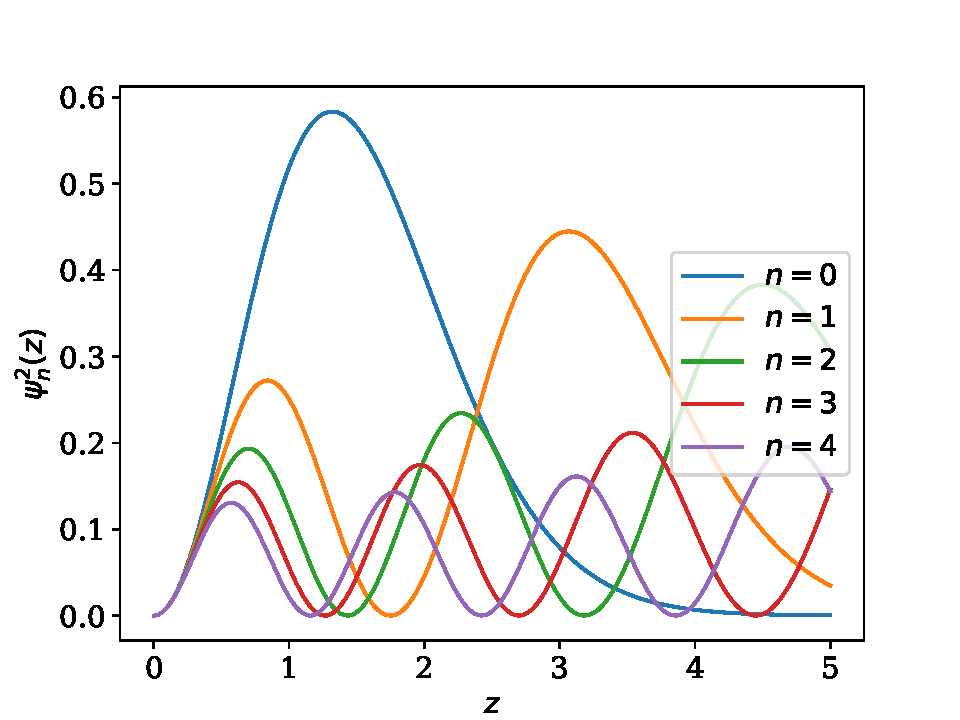
\includegraphics[angle=0,width=15cm ]{finite-size/etats-laser.pdf}
\caption{The scaled probability density function $p(z)$ for the distribution of the height at
a single point for the Airy line given in Eq. (\ref{airyprob})}
\label{1dpot}
\end{center}
\end{figure}
Using this we find the average height is given by
\begin{equation}
\langle h\rangle = \overline h= \ell z_0,
\end{equation}
where 
\begin{equation}
z_0 = \frac{\int_0^\infty dz z {\rm Ai}^2(z-\alpha_1)}{\int_0^\infty dz {\rm Ai}^2(z-\alpha_1)}.
\end{equation}
Interestingly comparison with the thermodynamic calculation giving Eq. \eqref{h1} shows that the identity
\begin{equation}
z_0 = \frac{2}{3}\alpha_1,
\end{equation}
must hold- this surprising identity can be verified numerically. Here we find that the average height given by
\begin{equation}
\langle h\rangle= 0.697089 \ \ell.
\end{equation}
The variance of the magnetisation is then given by
\begin{eqnarray}
\langle M^2\rangle_c &=& -TL\frac{\partial^2}{\partial \lambda^2}f (\lambda)|_{\lambda=0}=-TL\frac{\partial^2}{\partial P^2}f (P)|_{P=P_0}\\
&=& L\frac{\alpha_1 }{2^\frac{1}{3} \sigma^\frac{1}{3}\beta^\frac{5}{3}}\frac{2}{9}P_0^{-\frac{4}{3}}.
\end{eqnarray}
In terms of the average height this then gives
\begin{equation}
\langle M^2\rangle_c = \frac{9}{4\alpha_1^3}L\sigma\beta \overline h^4
\end{equation}


%%%%%%%%%%%%%%%%%%%%
\section{The generalized Lopes-Jacquin-Holdsworth Method}
\label{gen-lopes}
%%%%%%%%%%%%%%%%%%%%
{\color{blue}
In Sec \ref{sec-lopes}, we have shown a way to numerically compute the free energy of a system at a chemical potential $\mu$ in absence of another potential. Here we generalise the method for any kind of external potential. We will explain the method for the Ising model, but the derivation for the SOS model is straightforward.

For any external field which can be written as $\mu V(\sigma)$, where $V(\sigma)$ is a function of the internal microscopic variables $\sigma_i$,  the Hamiltonian of the Ising model is
\begin{align}
H = - J \sum_{} \sigma_i \sigma_j - \mu \sum_i V(\sigma_i)
\end{align}
The mean value of the external potential is
\begin{align}
    <  \sum_i V(\sigma_i) > =&  \sum_{\bf h} \sum_i V(\sigma_i) \exp(-\beta H) \nn
    =&  - \frac{\partial F(\mu)}{\partial \mu}
\end{align}
where $F$ is the free energy of the system. We see that for any potential of the form \eqref{lopes-gen}, we can integrate the previous equation to find
\begin{align}
   F(\mu_1) - F(\mu_2) = - \int_{\mu_1}^{\mu_2} d\mu'  < \sum_i V(\sigma_i) >_{\mu'} 
   \label{lopes-gen}
\end{align}

In the case where we know the analytical form of the free energy in the limits $\mu_2 \to \infty$ or $\mu_1 \to 0$, this method provides a way to directly measure it for any temperature or size by integrating over the chemical potential.
From the total free energy, we recover the Casimir form through Eq \eqref{cas-lopes}.
The limit $\mu_1 \to 0$ is the free system limit, and the free energy can not be computed analytically. However, when $\mu_2 \to \infty$, for  the majority of external fields $V(\sigma)$ in which we are interested, there is often a configuration limit whose free energy can be computed analytically. For example, if $V(\sigma)=\sigma$, the configuration limit is the one where all spins point towards the same direction, leading to a free energy of $0$. Thus, we have
\begin{align}
   F(\mu_1) - F_{analytic}(\infty) = - \int_{\mu_1}^{\infty} d\mu'  < \sum_i V(\sigma_i) >_{\mu'} 
   \label{lopes-gen}
\end{align}
In numerical simulations, it is not possible to range over infinity, and a criterion has to be defined to know the error made between the analytic case $\mu_2 = \infty$ and the maximal $\mu_2$ achieved in simulations. As in Eq \eqref{function-d}, we define the function
\begin{align}
    D(\mu,L_1,L_2) =  < M^\ast(L_1)-M^\ast(L_1-1) - (M^\ast(L_2)-M^\ast(L_2-1) >
\end{align}
with the generalized magnetization $M^\ast = \sum_i V(\sigma_i)$. A suitable upper limit of integration if we want to get the Casimir force is when the function $D$ reaches $0$ within the precision of the simulation.


For the SOS Hamiltonian
\begin{align}
    H =  J \sum_i |h_i -h_{i+1}|  + \mu \sum_i V(h_i)
\end{align}
we define the generalised mean height as
\begin{align}
    h^\ast = < \sum_i V(h_i) >
\end{align}
Eqquation \eqref{lopes-gen} writes as
\begin{align}
   F(\mu_1) - F(\mu_2) = -  \int_{\mu_1}^{\mu_2} d\mu' h^\ast(\mu')
   \label{diff-gene}
\end{align}
which can be directly be verified with the transfer matrix. 
In the limit $\mu \to \infty$, the generalised height is zero, while the free energy $F(\infty)$ can often be computed analytically. 
To minimize the error between the analytical limit and the numerical simulations, a suitable choice of the upper integration's limit $\mu_2$ is given by
\begin{align}
    \int_{\mu_2}^\infty  d\mu' h^\ast(\mu')) \ll \int_{\mu_1}^{\mu_2}  d\mu' h^\ast(\mu')
\end{align}
An heuristic argument to find a suitable upper limit for integration is when $h^\ast(\mu_2) \ll h^\ast(\mu_1)$.
In Fig \ref{integration-free-ene}, we see the free energy computed from the matrix transfer, compared to the integration procedure \eqref{lopes-gen} for the SOS model for the chemical potential $V(h_i)=h_i$ in Monte Carlo simulations, where we see the agreement for $\mu_2$ large enough.

\begin{figure}
    \centering
    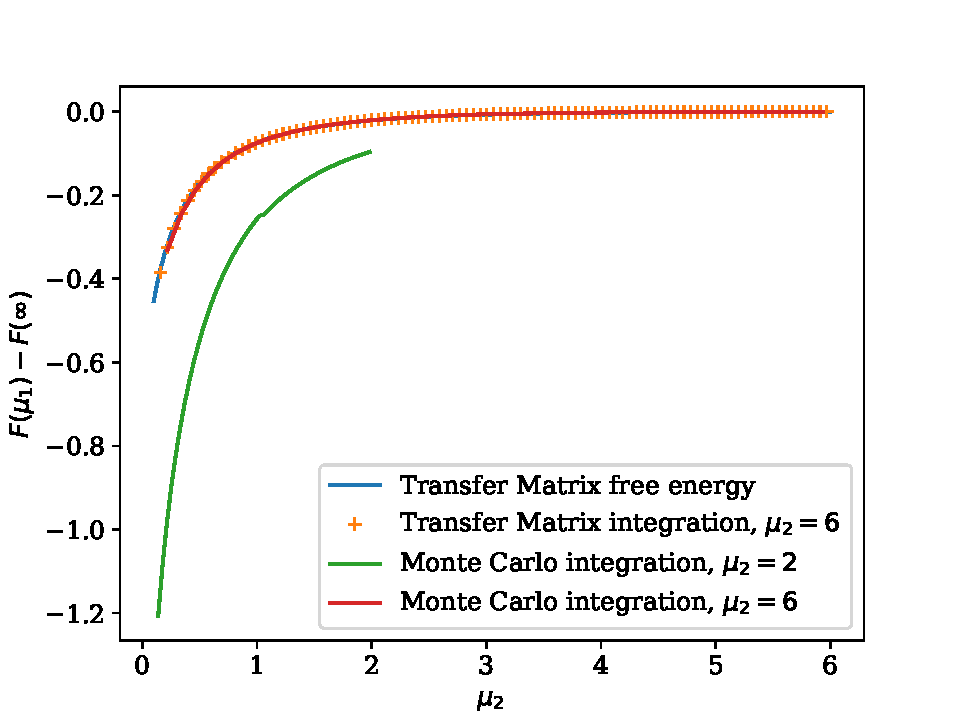
\includegraphics[width=0.7\linewidth]{int-dyn/integration-free-ene.pdf}
    \caption{Difference in free energy directly computed from transfer matrix, compared to numerical integration over the generalized height, for different upper limit $\mu_2$. The parameters are $L' = 256$, $L=200$ and $\beta=1$ for $5e7$ Monte Carlo steps.}
    \label{integration-free-ene}
\end{figure}

Since the order parameter is conserved in model B, the generalized Lopes-Jacquin-Holdswroth method can be used to compute the free energy for Kawasaki dynamics for potentials different from the chemical potential. 
As a proof of concept, we take a potential of the form
\begin{align}
    V(h_i) = - |h_i-\frac{L}{2}|
    \label{neggstaged}
\end{align}
Such potential will press the interface along $h=0$ and $h=L$ compared to the classical chemical potential which presses the interface at $h=0$, as seen in Fig \ref{fig-negstagged}. Far away from $\frac{L}{2}$, both potentials are equivalent in symmetric fashion, and shall behave similarly for large $\mu$, because the free energy only depends on the interface fluctuations and not the mean height. 


\begin{figure}
    \centering
	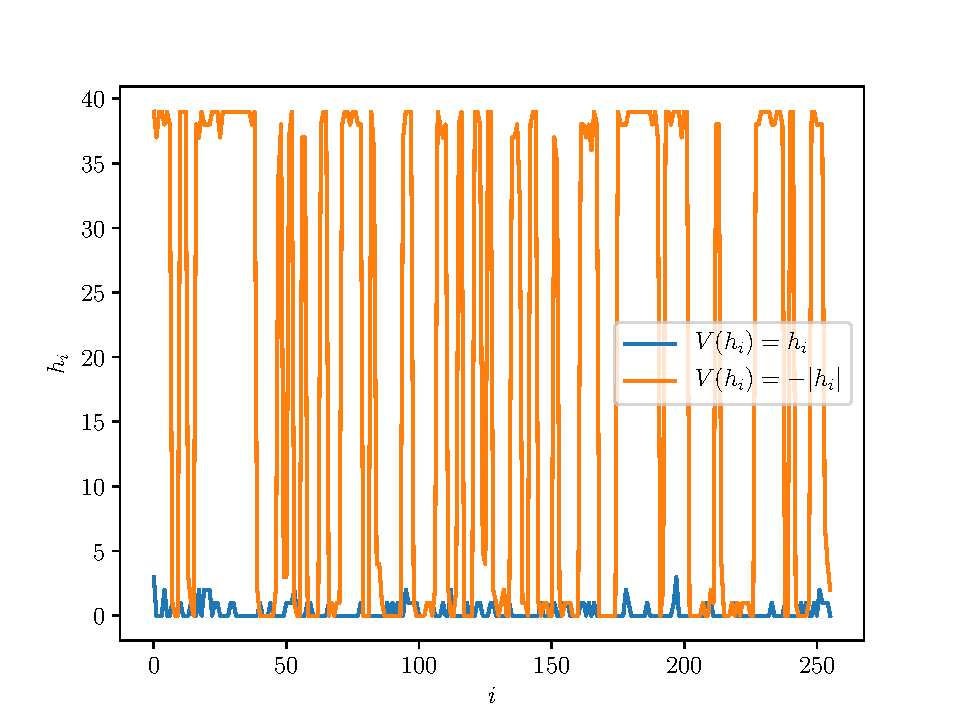
\includegraphics[width=0.7\linewidth]{int-dyn/comp-potentiels-chimiques.pdf}
	\caption{Snapshots of systems for the potential \eqref{neggstaged} and the chemical potential for $\beta=1$ and $\mu=2$ with $L=40$ and $L'=256$}
    \label{fig-negstagged}	
    \centering
   	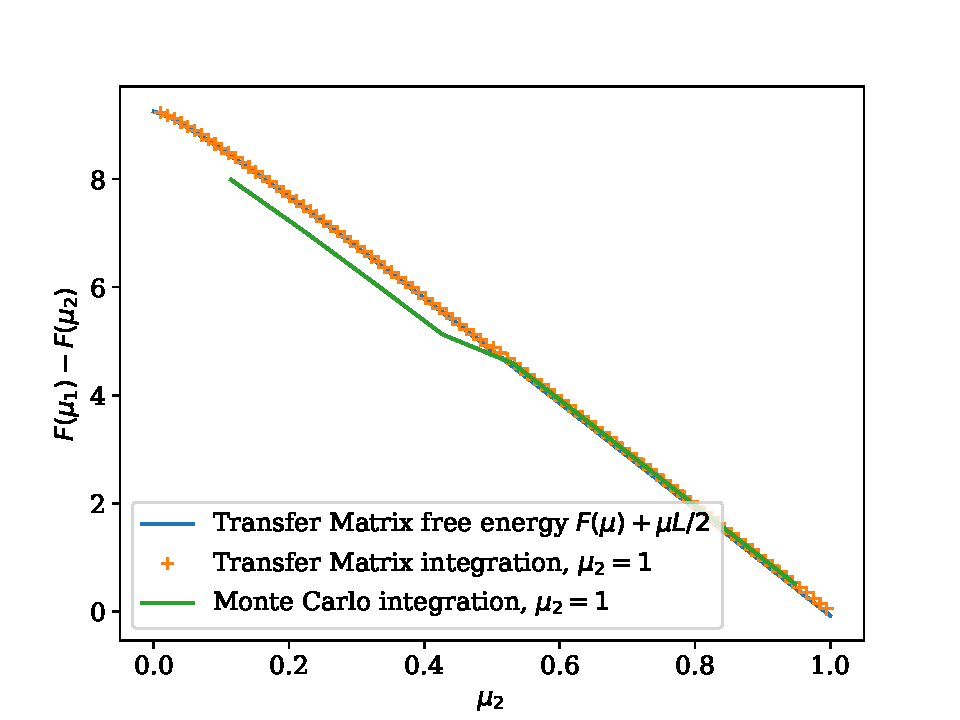
\includegraphics[width=0.7\linewidth]{int-dyn/integration-free-ene-negstagged.pdf}
    \caption{Difference in free energy directly computed from transfer matrix with the potential \eqref{neggstaged}, compared to numerical integration over the generalized height. The parameters are $L' = 256$, $L=20$ and $\beta=1$, $\mu_2 = 1$for $10^7$ Monte Carlo steps. } 
   	\label{fig-int-negstagged}    
\end{figure}  

In the $\mu \rightarrow \infty$ limit, the system has two equilibrium positions $h=0$ et $h=L$, which gives the transfer matrix
\begin{align}
T= e^{\beta \mu \frac{L}{2}}
  \begin{pmatrix}
    1 & e^{-\beta  J L} \\
    e^{-\beta  J L} & 1
  \end{pmatrix}
\end{align}
The eigenvalues are $\lambda_\pm = e^{ \beta \mu \frac{L}{2}}( 1 \pm e^{-\beta J L})$, which gives us the free energy 
\begin{align}
  F(\mu \rightarrow \infty) = - \mu \frac{L}{2}
\end{align}
We plotted in Fig \ref{fig-int-negstagged} the difference of free energy computed from the transfer matrix between $\mu_1$ finite and $\mu_2=1$, and the integration procedure \eqref{diff-gene} with the generalized height with the matrix transfer and Monte Carlo simulations, both for Glauber and Kawasaki dynamics. The disagreement between the expected value and the simulation results are from a $\mu_2$ too small, which we also see in the integration of the generalized height from the transfer matrix. We can convince ourselves by doing the integration from the transfer matrix for a larger $\mu_2$. Also, it is worth noting that for this system, there is no significant difference in results for the two different dynamics.

This method opens a new way to compute the free energy for any kind of external potential of the form $\mu V(h)$, or $\mu V(\sigma)$ in the case of the Ising or SOS models for conserved and non-conserved dynamics, such as non-uniform external fields \cite{bissacot_phase_2010}. 
}


%%%%%%%%%%%%%%%%%%%%
\section{The confined solid on solid model}
%%%%%%%%%%%%%%%%%%%%

{\color{blue}
From exact diagonalization of the SOS transfer matrix in the infinite case \cite{guyer_sine-gordon_1979}, finite-size effects were studied both for the SOS and RSOS model \cite{svrakic_finite-size_1988,privman_finite-size_1988}. Nevertheless the derivation of eigenvectors and eigenvalues were not explicit in the latter case. Those eigenvalues are a multiple of an integer, and the study of the eigenvalues issued from an odd integer where also not discussed. We also add an analysis to the correlation length and the limits of high and low temperatures for the free energy. 

We consider here the free interface confined between $0$ and $L$, with no external field.} {\color{red} The SOS transfer matrix is thus given by 
\begin{align}
T(h_i,h_j) = \exp(-\beta J |h_i-h_j|)
\end{align}
Since positions are comprised from $0$ to $L$, we can write the transfer matrix as}
\begin{equation}
T_{ij} = \exp(-\beta J|i-j|).
\end{equation}
We introduce 
\begin{equation}
r=\exp(-\beta\ J)
\end{equation}
To find the eigenvectors of $T$, we consider the vector denoted by $[a]$ which has components
\begin{equation}
[a]_i = a^i,
\end{equation}
where $i$ is an index ranging from $0$ to $L$. 
The action of the SOS transfer matrix on this vector is given by
\begin{equation}
\left[T\ [a]\right]_i = \sum_{j=0}^L r^{ |i-j|} a^j
\end{equation}
and we find
\begin{align}
[T\ [a]]_i
=& r^i \sum_{j=0}^i r^{-j} a^j + r^{-i} \sum_{j= i+1}^L r^j a^j \nn
=& r^i \sum_{j=0}^i r^{-j} a^j + r^{-i} \sum_{k= 0}^{L-i-1} r^{i+1+k} a^{i+1+k} \nn
=& r^i \frac{1- r^{-(i+1)} a^{i+1}}{1- r^{-1} )a} + r a^{i+1}\frac{1- r^{L-i} a^{L-i}}{1- r a} \nn
=&\left[\frac{ ra}{1-ra}- \frac{ \frac{a}{r}}{1-\frac{a}{r}}\right]a^i +\frac{r^i}{1-\frac{a}{r}}-\frac{r^{L+1-i}a^{L+1}}{1-ra}
\end{align}
We now define
\begin{equation}
\lambda(a)= \frac{ ra}{1-ra}- \frac{ \frac{a}{r}}{1-\frac{a}{r}} = \frac{\frac{1}{r}-r}{\frac{1}{r}+r
- a-\frac{1}{a}}
\label{elam}
\end{equation}
and notice that
\begin{equation}
\lambda(a) = \lambda(a^{-1})
\end{equation}
We can thus write
\begin{equation}
[T\ [a]]_i= \lambda(a)a^i +\frac{r^i}{1-\frac{a}{r}}-\frac{r^{L+1-i}a^{L+1}}{1-ra}
\end{equation}
Now, considering the action of the transfer matrix on the vector $[a^{-1}]$, we find
\begin{equation}
\left[T\ [a^{-1}]\right]_i = \lambda(a) a^{-i} + \frac{r^i}{1-\frac{1}{ra}}-\frac{r^{L+1-i}a^{-(L+1)}}{1-\frac{r}{a}}
\end{equation}
We now look for an eigenvector of the form
\begin{equation}
{\bf v} = [a]+ c[a^{-1}]
\end{equation}
The action of $T$ on ${\bf v}$ is 
\begin{equation}
\left[T\ ([a]+c [a^{-1}]\right]_i = \lambda(a)[a^i + c a^{-i}]
+ r^i\left(\frac{1}{1-\frac{a}{r}}+ \frac{c}{1-\frac{1}{ra}}\right)
- r^{L+1-i} \left(\frac{a^{L+1}}{1-ra} + c\frac{a^{-(L+1)}}{1-\frac{r}{a}}\right)
\end{equation}
and we see that ${\bf v}$ is an eigenvector, with eigenvalue $\lambda(a)$, if
\begin{eqnarray}
\frac{1}{1-\frac{a}{r}}+ \frac{c}{1-\frac{1}{ra}}&=&0 \\
\frac{a^{L+1}}{1-ra} + c\frac{a^{-(L+1)}}{1-\frac{r}{a}} &=& 0
\end{eqnarray}
The above equations imply that 
\begin{equation}
c= -\frac{ra-1}{a(r-a)}
\end{equation}
and
\begin{equation}
c^2 = a^{2L}
\end{equation}
Therefore we find
\begin{equation}
v_i = a^i \pm a^{L-i}
\end{equation}

\subsubsection*{Ground state eigenvector}
We expect the ground state eigenvector (corresponding to the largest eigenvalue) to be symmetric with respect to the middle of the system and so 
\begin{equation}
v_i= v_{L-i}
\end{equation}
which implied that we should have $c= a^L$. 

This then gives the equation determining the values of a for the largest eigenvalue, and in general for the eigenvalues which are symmetric ( $c=1$),
\begin{equation}
a^{L+1} = \frac{1-ra}{r-a}.
\label{aeq}
\end{equation}

As a check on the above derivation we can consider the case $L=1$ so we have two sites. Here we see that the transfer matrix is given explicitly by
\begin{equation}
T =\begin{pmatrix} & 1 & r\\& r &1\end{pmatrix}
\end{equation}
and the largest eigenvector is easily seen to be given by
\begin{equation}
\lambda_0 = 1+r 
\end{equation}
In this case, we seethat Eq. (\ref{aeq}) gives
\begin{equation}
a^{2} = \frac{1-ra}{r-a}
\end{equation}
which has three solutions
\begin{eqnarray}
a_1&=& -1\\
a_2&=& \frac{1}{2} \left(-\sqrt{r^2+2
r-3}+r+1\right) \\
a_3&=& \frac{1}{2} \left(\sqrt{r^2+2
r-3}+r+1\right)\end{eqnarray}
We see that $a_2=1/a_3$, and $|a_2|=|a_3|=1$, and that
\begin{equation}
\lambda(-1)= \frac{1-r}{1+r}
\end{equation}
while 
\begin{equation}
\lambda(a_2)=\lambda(a_3)= 1+r
\end{equation}
corresponds to the maximal eigenvalue. Note that $\lambda(-1)$ is not the other eigenvalue of the transfer matrix, this has to be found by considering solutions with $c=-1$, as we will see later.

The equation (\ref{aeq}) determining $a$ can also be written as
\begin{equation}
a^{L} = - \frac{r-\frac{1}{a}}{r-a}
\end{equation}
From this we see that if $a$ is a solution then $1/a$, and that $a=-1$ is always a solution.


We now introduce $\theta$ and 
\begin{align}
a=\exp(i\theta)
\label{def-theta}
\end{align}
Then the parameter of the eigenvector is
\begin{equation}
\exp(i L \theta) = - \frac{r-\exp(-i\theta)}{r-\exp(i\theta)}
\label{thetamas}
\end{equation}
From Eq \eqref{elam}, we have
\begin{equation}
\lambda(\theta) = \frac{\sinh(\beta J)}{\cosh(\beta J) - \cos(\theta)}.
\end{equation}
Notice that in order to construct a real eigenvector corresponding to $\lambda_0$ we can use the fact that both $v_i(a) = a^i + a^{L-i}$ and $v_i(a^{-1}) = a^{-i} + a^{-L+i}$ are both eigenvectors with the same eigenvalue. This means that $u_i(a) = v_i(a) + v_i(-a)$ is also an eigenvector and all its components are real. 

Clearly the largest eigenvalue corresponds to the value of $\theta$ closest to $0$,  so we look for an eigenvalue such that $L \theta \sim 1$. We write
\begin{equation}
\phi = L \theta
\end{equation}
For $L$ large, this gives
\begin{equation}
\exp(i\phi) \approx -\frac{r-1+ i\frac{\phi}{L}}{ r-1- i\frac{\phi}{L}}\approx -1 +2 i\frac{\phi}{L(1-r)}
\end{equation}
and so we find to leading order in $1/L$
\begin{equation}
\theta = \frac{(2n+1)\pi}{L}
\end{equation}
However we notice that this approximation is only valid if $L(1-r) \gg1$. For large $\beta$ this approximation is simply equivalent to $L\gg1$, however when $\beta$ is small it requires
that $H \beta \gg 1$.

The closest eigenvector to the real axis has $n=0$ and so we have
\begin{equation}
\lambda_0 \approx \frac{\sinh(\beta J)}{\cosh(\beta J) - \cos(\frac{\pi}{L})} \approx \frac{\sinh(\beta J)}{\cosh(\beta J) - 1+ \frac{\pi^2}{2 L^2}} \approx \coth(\frac{\beta J}{2})(1 - \frac{\pi^2}{4\sinh^2(\frac{\beta J}{2}) L^2})
\label{ground-sos}
\end{equation}
{\color{red} In the limit $L\to \infty$, the ground-state eigenvalue is the same as the Sine-Gordon chain of length $L' \to \infty$ fixed at $h(0) = h(L') = 0$ and using a SOS interaction between nearest neighboors \cite{guyer_sine-gordon_1979}, which is normal since boundary conditions on the x-axis are negligible in the thermodynamic limit.}

\subsubsection*{First excited state eigenvector}
In order to compute the second eigenvalue $\lambda_1$ we look for an odd or antisymmetric solution with $c=-1$. We thus find
\begin{equation}
\exp(i L\theta) = \frac{r-\exp(-i\theta)}{r-\exp(i\theta)}
\label{theta}
\end{equation}

For large $L$ we look for a solution of the form $\theta=\phi/L$ and this gives
\begin{equation}
\exp(i\phi) \approx 1
\end{equation}
and so we chose solutions $\phi = 2n\pi$ for integer $n$. However the solution $n=0$ which corresponds to $a=1$ has $v(i) = a^i-a^{L-i} =0$ and so does not correspond to an eigenvector. We thus take the next solution $\phi = 2\pi$ which gives
\begin{equation}
\lambda_1 \approx \frac{\sinh(\beta J)}{\cosh(\beta J) - \cos(\frac{2\pi}{L})} \approx \frac{\sinh(\beta J)}{\cosh(\beta J) - 1+ \frac{2\pi^2}{L^2}}\approx \coth(\frac{\beta J}{2})(1 - \frac{\pi^2}{\sinh^2(\frac{\beta J}{2}) L^2})
\label{excited-sos}
\end{equation}
In Fig \ref{large-l-limit}, we show the agreement between the computation of the first two eigenvalues !!!! computed by numerical diagonalisation and compared with the analytical approximations Eq. \eqref{ground-sos} and Eq. \eqref{excited-sos} which are valid for the large L limit
\begin{figure}
\centering
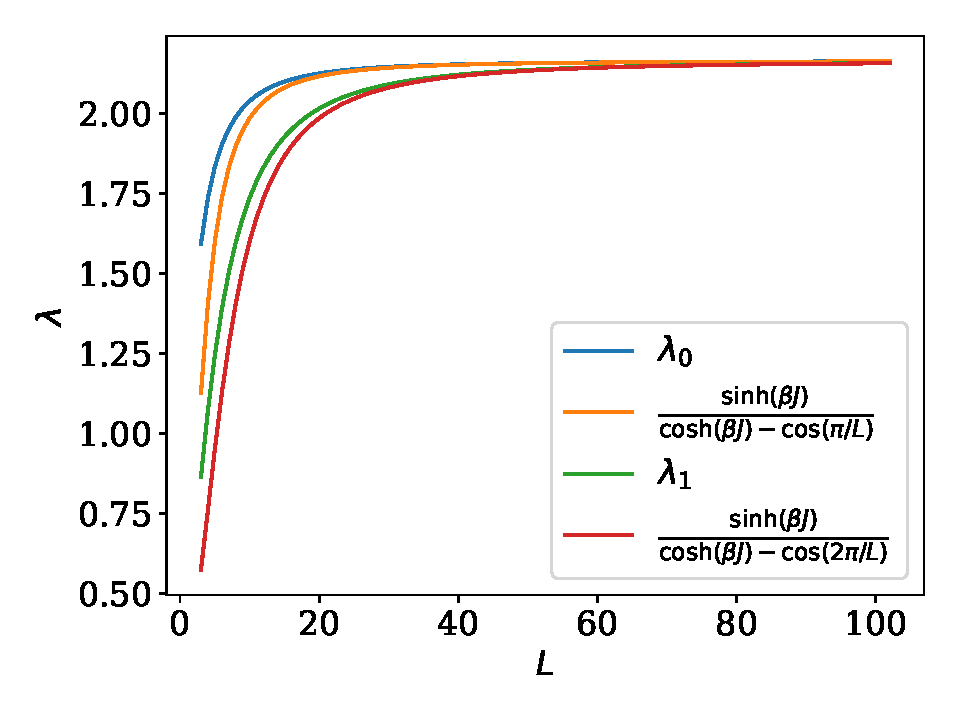
\includegraphics[width=0.7\linewidth]{finite-size/null_deanJ.pdf}
\caption{$\lambda_0$ and $\lambda_1$ as a function of $L$ computed by numerical diagonalisation of the transfer matrix, compared to the analytical approximations for large $L$: Eq. \eqref{ground-sos} and Eq. \eqref{excited-sos}. Here we have chosen  for $J=1$ and $\beta=1$.}
\label{large-l-limit} 
\end{figure}

The correlation length is then given by
\begin{equation}
\xi =\frac{1}{\ln(\frac{\lambda_0}{\lambda_1})} = \frac{1}{\ln(\frac{\cosh(\beta J) - \cos(\frac{\pi}{L})}{\cosh(\beta J) - \cos(\frac{2\pi}{L})})}\approx \frac{4}{3}\frac{\sinh^2(\frac{\beta J}{2})L^2}{\pi^2}
\end{equation}
and we see that this has the same form as that for the free elastic line in Eq. (\ref{corel}).
Furthermore, the free energy per site is given in the thermodynamic limit and for large $L$ by
\begin{equation}
f=-\frac{1}{\beta}\ln(\lambda_0) \approx -\frac{1}{\beta}\left[ \ln(\coth(\frac{\beta J}{2}))- \frac{\pi^2}{4\sinh^2(\frac{\beta J}{2}) L^2}\right]
\end{equation}
and this gives a pressure
\begin{equation}
P= -\frac{\partial f}{\partial L}= \frac{T\pi^2}{2 \sinh^2(\frac{\beta}{2}) L^3}
\end{equation}


This has the same form as the pressure for the elastic line in Eq. \eqref{pfree} if we make the identification of the effective surface tension to be used in the elastic line model
\begin{equation}
\sigma_{eff} = \frac{2}{\beta}\sinh^2(\frac{\beta J}{2})
\end{equation}
We should note that this is also consistent with the equality deduced by comparing the correlation length of the two models.

We see that in the limit of large $L$ and for appropriately low temperatures, the finite size SOS model reproduced the phenomenology of the elastic line (confined Edwards-Wilkinson surface). 
This is not surprising as a low temperatures jumps of more that two lattice spacings in the height are suppressed by a factor or $\exp(-\beta J)$ with respect to staying at the same height moving up or down by one site. The low temperature SOS model thus becomes effectively equivalent to the RSOS model and thus is equivalent to a local random walk model. 

\subsubsection*{High temperature limit}

To explore the high temperature limit we can note that if we write
\begin{equation}
z= r-\exp(-i\theta)
\end{equation}
we can write Eq. \eqref{thetamas} as
\begin{equation}
\exp(i L\theta) = -\frac{z}{\overline z} = \exp(2i\psi + i\pi)
\end{equation}
where
\begin{equation}
\tan(\psi) = \frac{\sin(\theta)}{r-\cos(\theta)}
\end{equation}
This then gives 
\begin{equation}
L \theta = 2\psi + \pi
\end{equation}
and so
\begin{equation}
\tan(\psi) = \frac{\sin(\theta)}{r-\cos(\theta)}= \tan(\frac{L\theta}{2} +\frac{\pi}{2})= - \cot(\frac{L\theta}{2})
\end{equation}
which finally gives
\begin{equation}
\tan(\frac{L\theta}{2}) = \frac{\cos(\theta)-r}{\sin(\theta)}
\label{mde}
\end{equation}
In this form we see that our calculations agree with those of Svravick et al \cite{svrakic_finite-size_1988}. Futhermore when $\beta\to 0$ we know that the elements of the transfer matrix all tend to one and that the largest eigenvalue has all components equal. This means that in the infinite temperature limit, $\theta=0$. Therefore in Eq. \eqref{mde} we look for solutions where $\theta$ is small. Taylor expanding gives to leading order
\begin{equation}
\frac{L\theta^2}{2} \approx1-r-\frac{\theta^2}{2}
\end{equation}
which gives
\begin{equation}
\theta \approx \sqrt{\frac{2(1-r)}{L+1}}
\end{equation}
However the above expansion assumes that $\theta L\ll1$ and so
\begin{equation}
\sqrt{2L(1-r)} \ll 1
\end{equation}
This means that the height can fluctuate by of order $L$ from site to site. The high temperature approximation is thus equivalent to
\begin{equation}
\theta \approx \sqrt{\frac{2\beta J}{L+1}}.
\end{equation}
Therefore at high temperature this means that $L \beta J\ll1$. 
This gives a maximal eigenvalue
\begin{equation}
\lambda_0 = L+1
\end{equation}
and the free energy
\begin{equation}
f=-\frac{1}{\beta}\ln(L+1)
\end{equation}
which is the obvious result coming from the infinite temperature entropy. 
This result suggests that the solution for $\theta$ at small $\beta$ can be written as a perturbation series of the form
\begin{equation}
\theta = \sqrt{\beta J}\sum_{n=0}^\infty b_n (\beta J)^n
\end{equation}
The first two terms give
\begin{equation}
\theta = \sqrt{\beta J}\left[\sqrt{\frac{2\beta J}{L+1}} -\beta J \frac{2 + 2L +L^2}{6\sqrt{2}(1+L)^{\frac{3}{2}}}\right]
\end{equation}
and from this we find
\begin{equation}
f=-\frac{1}{\beta}\ln(L+1-\beta J\frac{L^2+2L}{3})
\label{high-temperature} 
\end{equation}
{\color{red} and where we show in Fig \ref{fig-high-temp} the agreement of the high-temperature approximation \eqref{high-temperature} with respect to the direct diagonalization of the transfer matrix.}
As pointed out above this result gives the high temperature entropy but it also exhibits the correct average energy $\epsilon$ per unit length at high temperature. To see this we note that all values of $h$ are equiprobable at infinite temperature and so
\begin{equation}
\epsilon = \frac{1}{(L+1)^2} J \sum_{i,j=0}^L |i-j| = J\frac{L^2+2L}{3}
\end{equation}

\begin{figure}
\centering
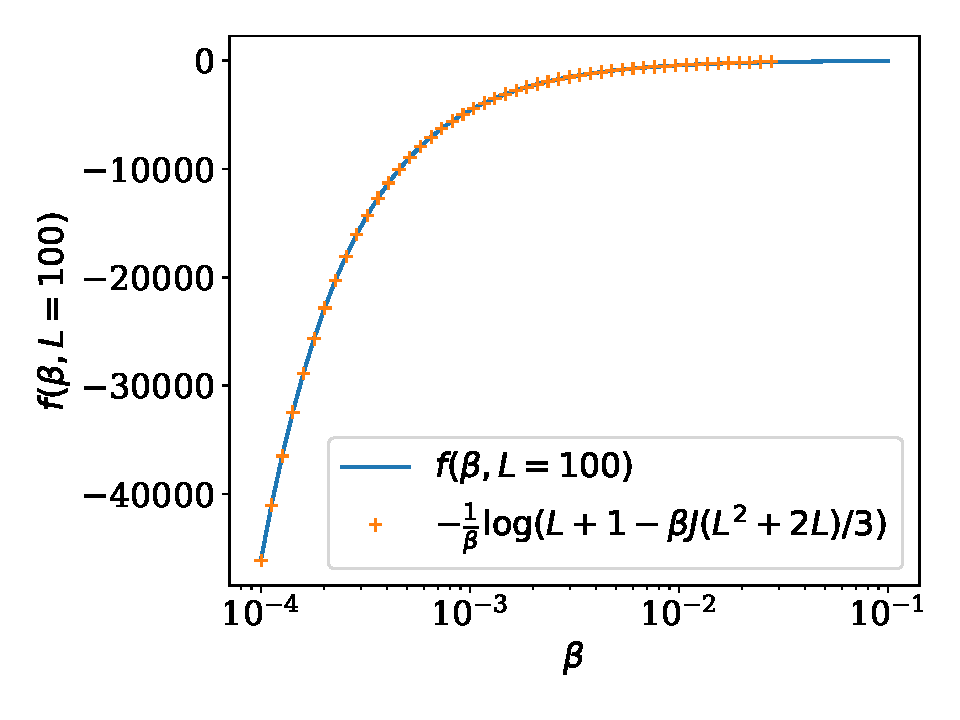
\includegraphics[width=0.7\linewidth]{finite-size/high_temperature.pdf}
\caption{Free energy with respect to $\beta$ for $L=100$ and $J=1$ in the high-temperature limit, by direct diagonalization of the transfer matrix and by Eq \eqref{high-temperature}.}
\label{fig-high-temp} 
\end{figure}


%%%%%%%%%%%%%%%%
\section{Conclusion}
%%%%%%%%%%%%%%%%

Finite-size effects corrections in the free energy become important when the correlation length becomes of the order of magnitude of the system's size. The derivative of the free energy with respect to the system size yields a confinement pressure. The electromagnetic field energy goes as $U_{int}(L) = -\frac{\hbar \pi^2 c A}{720 L^3}$ \cite{h_b_g_casimir_attraction_1948,sm_rytov_principles_1989,lifshits_theory_1955}, while for critical systems Fisher and de Gennes showed that  \cite{amit_field_2005}, it goes as $F(t=0) = \frac{k_B T A C}{L^{d-1}}$ \cite{gambassi_casimir_2009}.

The path integral method \cite{matsubara_new_1955} is well suited to the study of the Gaussian continuous interface model. We developed a general framework for the probability density function for height profile $h$ using the wavefunctions arising from the Schr\"odinger equation analysis of the path integral. In the thermodynamic limit, only the ground state  is relevant, giving the free energy per unit length $f= \frac{1}{\beta}\epsilon_0$, where $\epsilon_0$ is the ground state energy and the correlation length $\xi = \frac{1}{\epsilon_1-\epsilon_0}$. 
Applying this framework to the confined elastic line, we find that the free energy per unit length goes as $f = \frac{T^2 \pi^2}{2 \sigma L^2}$, where $\sigma$ is the surface tension of the interface or the stiffness of the interface. Using a conjecture \cite{privman_finite-size_1988-1} about the finite-size corrections on the surface tension, and setting, we have shown that the Casimir effect as predicted by Fisher and de Gennes can be recovered in these interface models. 
Another example where we have applied ths framework is the one where we apply a constant pressure to the interface with a hard wall below at $h=0$ but with non above as the applied pressure is sufficient to localise the interface. In this case the probability density function of the height distribution is given by $p(h) \propto Ai^2(\frac{h}{\ell}-\alpha_1)$, where $\ell$ is the characteristic length scale of the interface, and we  find the average height $<h> = \frac{2}{3}\frac{\alpha_1}{\left(2\sigma \beta^2 P_0 \right)^\frac{1}{3}}$.

For discrete  Solid-On-Solid models, the path integral cannot be directly applied, and methods adapted to discrete systems must be used. The first method is to compute the free energy through numerical simulations. By defining the generalized magnetization $M^\ast = \sum_i V(\sigma_i)$ in the Ising model, and the generalized height $h^\ast = \sum_i V(h_i)$ in the SOS model, we generalized the Lopes-Jacquin-Holdsworth method \cite{lopes_cardozo_critical_2014} for the direct computation of the free energy, when one of the limit configurations of the system with respect to their conjugated variable $\mu$ is. Since the LJH does not work for Kawasaki dynamics where the order parameter is conserved, we applied our generalized method for the potential $V(h) = - | h - \frac{L}{2}|$, showing that numerically that this generalisation allows on to  compute the thermodynamic force for more complex fields than the uniform magnetic field in the Ising model.

For the confined SOS interface, we followed \cite{svrakic_finite-size_1988} to obtain the exact eigenvalues and eigenvectors of the transfer matrix. This gives us the free energy $f = -\frac{1}{\beta} \left( f_{bulk} - \frac{\pi^2}{4 \sinh^2(\frac{\beta J}{2} L^2 } \right)$, which has the same form as the continuous confined elastic line. 
